\section{Data Acquisition \& Challenges}
\begin{frame}{}
    \LARGE Video Learning \& Generation: \textbf{Data Acquisition \& Challenges}
\end{frame}

\begin{frame}[allowframebreaks]{Data Acquisition}
    \begin{itemize}
        \item Video data can be acquired from various sources, including:
        \begin{itemize}
            \item \textbf{Cameras:} Digital cameras, smartphones, and webcams.
            \item \textbf{Drones:} Aerial footage for surveillance or mapping.
            \item \textbf{Webcams:} Live streaming or recorded video.
            \item \textbf{Public Datasets:} Pre-recorded videos available for research.
        \end{itemize}
        \item Key considerations in data acquisition:
        \begin{itemize}
            \item Quality of the recording device.
            \item Environmental conditions (lighting, weather).
            \item Ethical considerations (privacy, consent).
        \end{itemize}
    \end{itemize}
\framebreak
    \begin{itemize}
        \item \textbf{Modern sources for video data:}
        \begin{itemize}
            \item \textbf{User-generated content:} Platforms like YouTube and TikTok provide vast amounts of diverse video data.
            \item \textbf{Surveillance \& IoT:} Cameras embedded in city infrastructure, public spaces, and smart devices continuously capture video streams.
            \item \textbf{Automotive:} Dashcams and sensors in autonomous vehicles generate large-scale driving and traffic video datasets.
        \end{itemize}
        \item \textbf{Metadata and tags:} Videos are often accompanied by metadata (timestamps, GPS, tags) that facilitate search, retrieval, and organization.
    \end{itemize}
\framebreak
    \item \textbf{Popular Video Datasets:}
    \begin{itemize}
        \item \textbf{UCF101:} 13,000+ video clips covering 101 human action categories.
        \item \textbf{Kinetics-700:} 650,000 video clips annotated with 700 action classes.
        \item \textbf{ActivityNet:} Large-scale dataset with untrimmed videos for temporal action localization.
        \item \textbf{Something-Something v2:} Focuses on fine-grained, object-centric actions.
        \item \textbf{Ego4D:} Egocentric videos capturing daily activities from a first-person perspective.
    \end{itemize}
\framebreak
    \begin{figure}
        \centering
        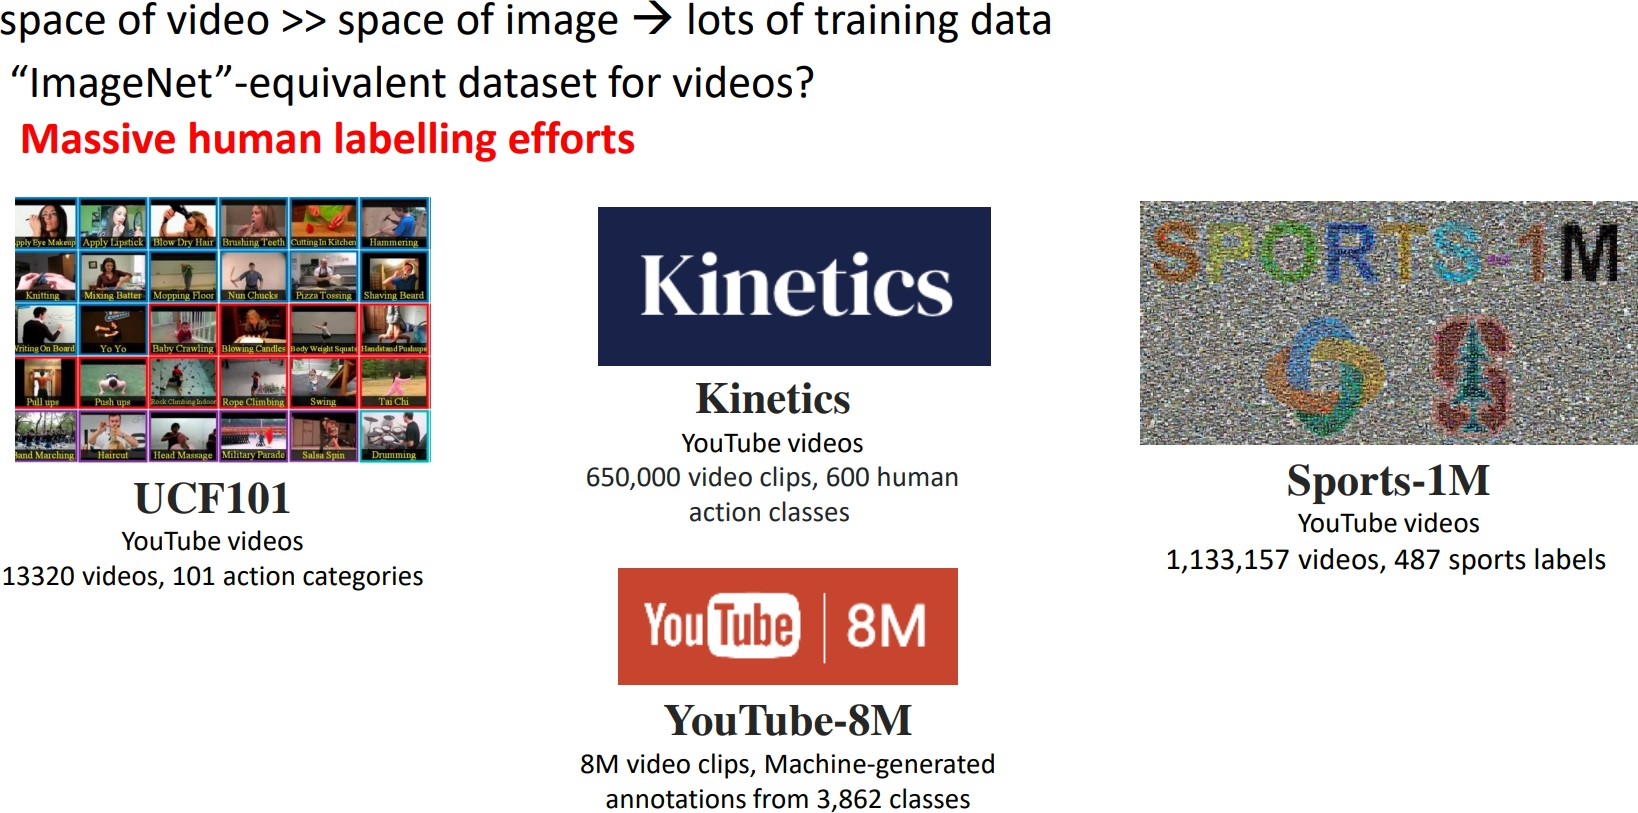
\includegraphics[width=1\textwidth,height=0.9\textheight,keepaspectratio]{images/video/slide_18_1_img.jpg}
    \end{figure}
\framebreak
    \begin{figure}
        \centering
        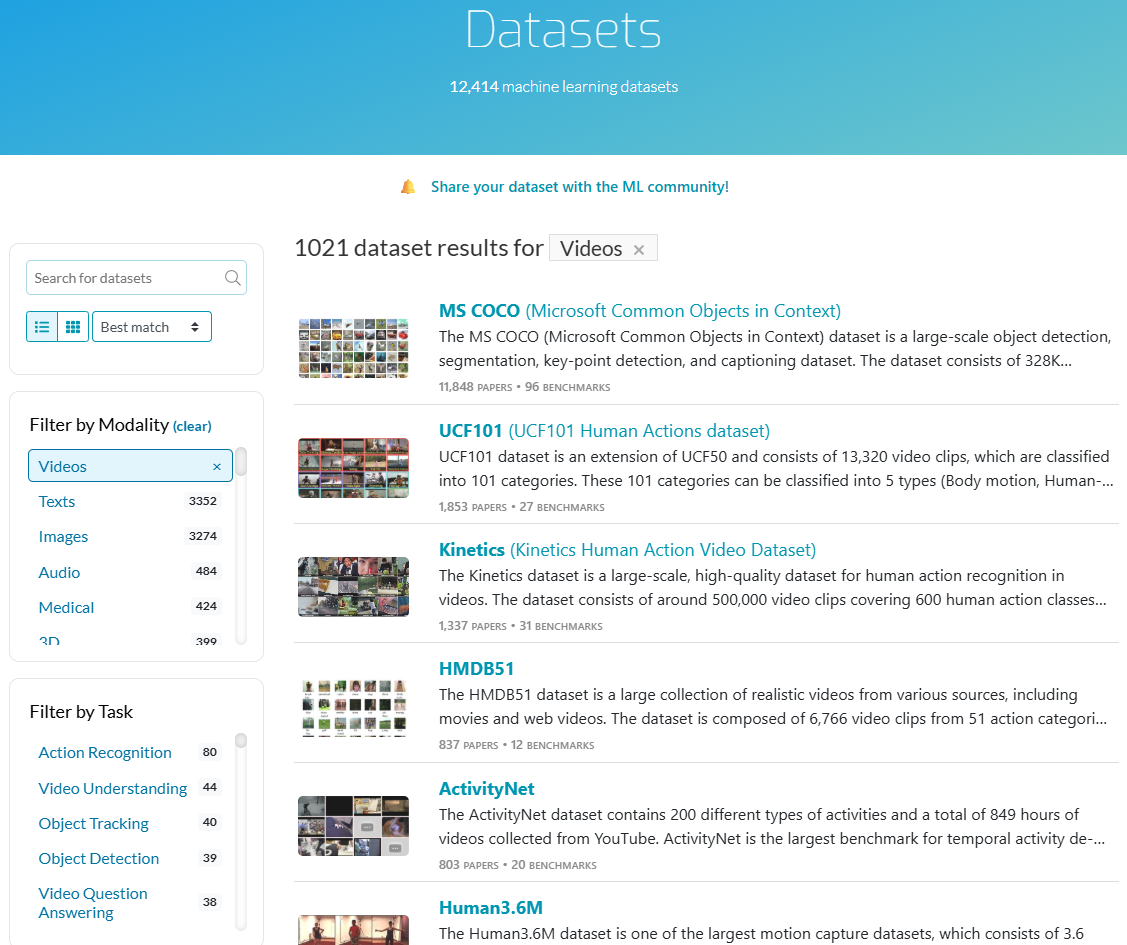
\includegraphics[width=1\textwidth,height=0.83\textheight,keepaspectratio]{images/video/dataset.png}
        \caption*{[Source: \url{https://paperswithcode.com/datasets?mod=videos}]}
    \end{figure}
\end{frame}

\begin{frame}[allowframebreaks]{Challenges in Video Data}
    \begin{itemize}
        \item \textbf{Issues Working with Videos:}
        \begin{itemize}
            \item \textbf{High Storage:} Video files are large, requiring significant storage and bandwidth.
            \item \textbf{Variable FPS \& Resolution:} Differences in frame rates and resolutions increase preprocessing complexity.
            \item \textbf{Annotation Cost:} Frame-level labeling is time-consuming and expensive.
            \item \textbf{Data Imbalance:} Rare events or classes are often underrepresented in datasets.
        \end{itemize}
    \end{itemize}
\framebreak
    \begin{figure}
        \centering
        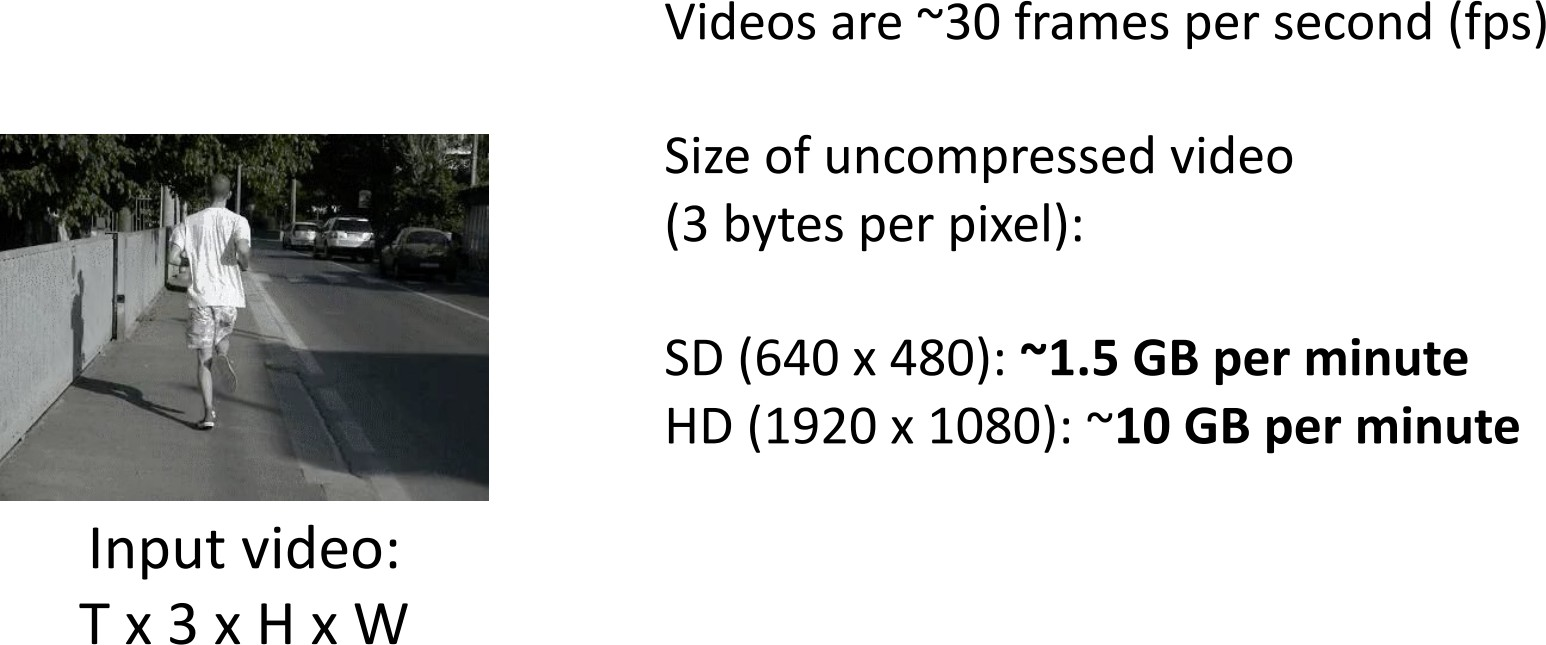
\includegraphics[width=1\textwidth,height=0.9\textheight,keepaspectratio]{images/video/slide_6_1_img.jpg}
    \end{figure}
\framebreak
    \begin{figure}
        \centering
        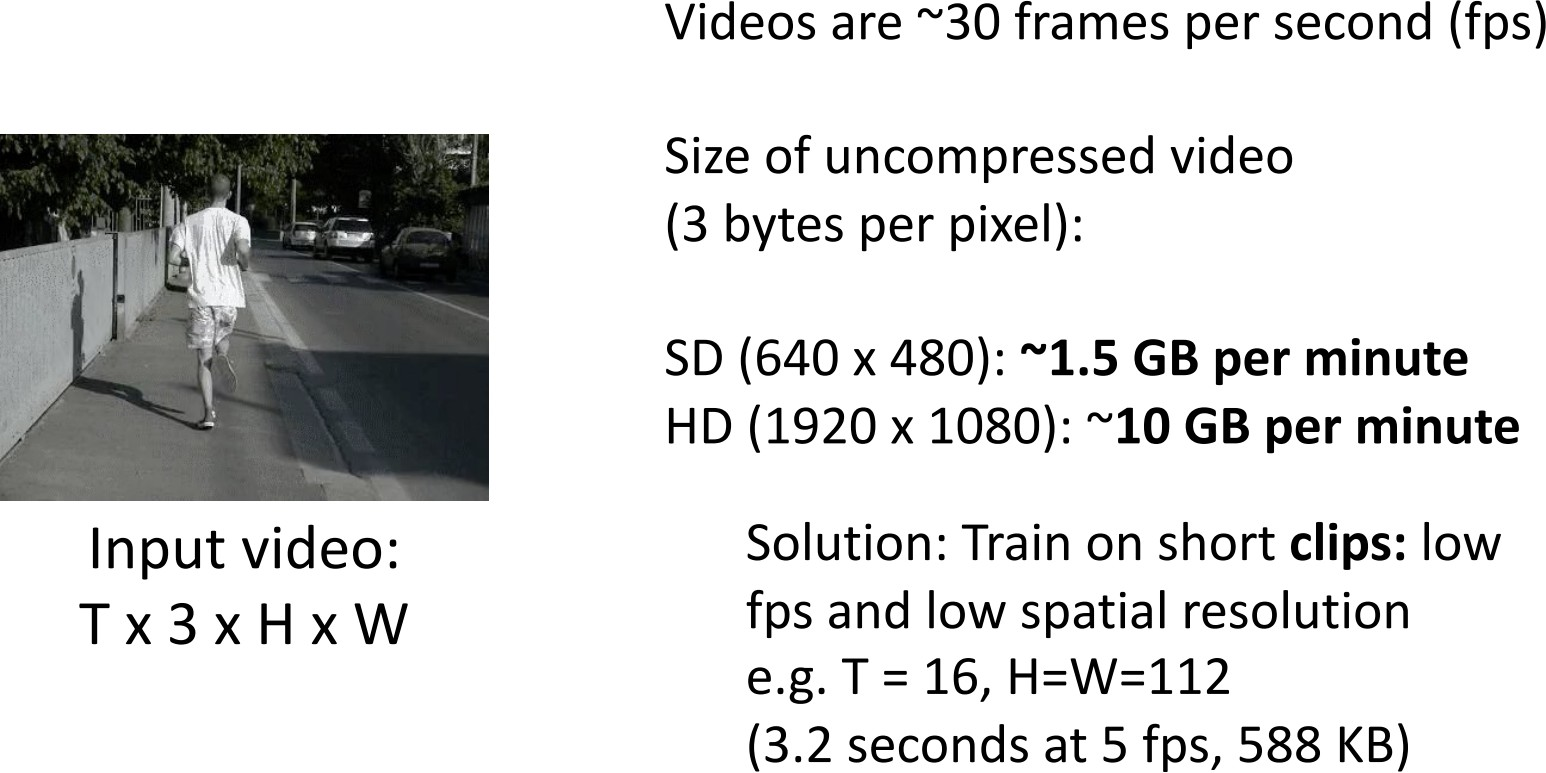
\includegraphics[width=1\textwidth,height=0.9\textheight,keepaspectratio]{images/video/slide_7_1_img.jpg}
    \end{figure}
\framebreak
    \begin{itemize}
        \item \textbf{Solutions for Video Data:}
        \begin{itemize}
            \item \textbf{Compression \& Sampling:} Techniques like keyframe extraction and frame sampling help reduce storage and computational requirements.
            \item \textbf{Data Augmentation:} Methods such as frame dropout and temporal jittering increase data diversity and robustness.
            \item \textbf{Synthetic Data:} Simulated environments (e.g., CARLA, AirSim) generate realistic video data for training and testing.
            \item \textbf{Weak \& Self-Supervision:} Leveraging unlabeled or partially labeled data reduces reliance on expensive manual annotations.
        \end{itemize}
    \end{itemize}
\end{frame}